%!TEX root = ../../thesis.tex


\section{ Updated Figueira 2016 results}
\todo{comparison of plots} figueira eta la plot 1, eniric plot

\begin{figure}
    \centering
    \begin{tabular}{cc}
        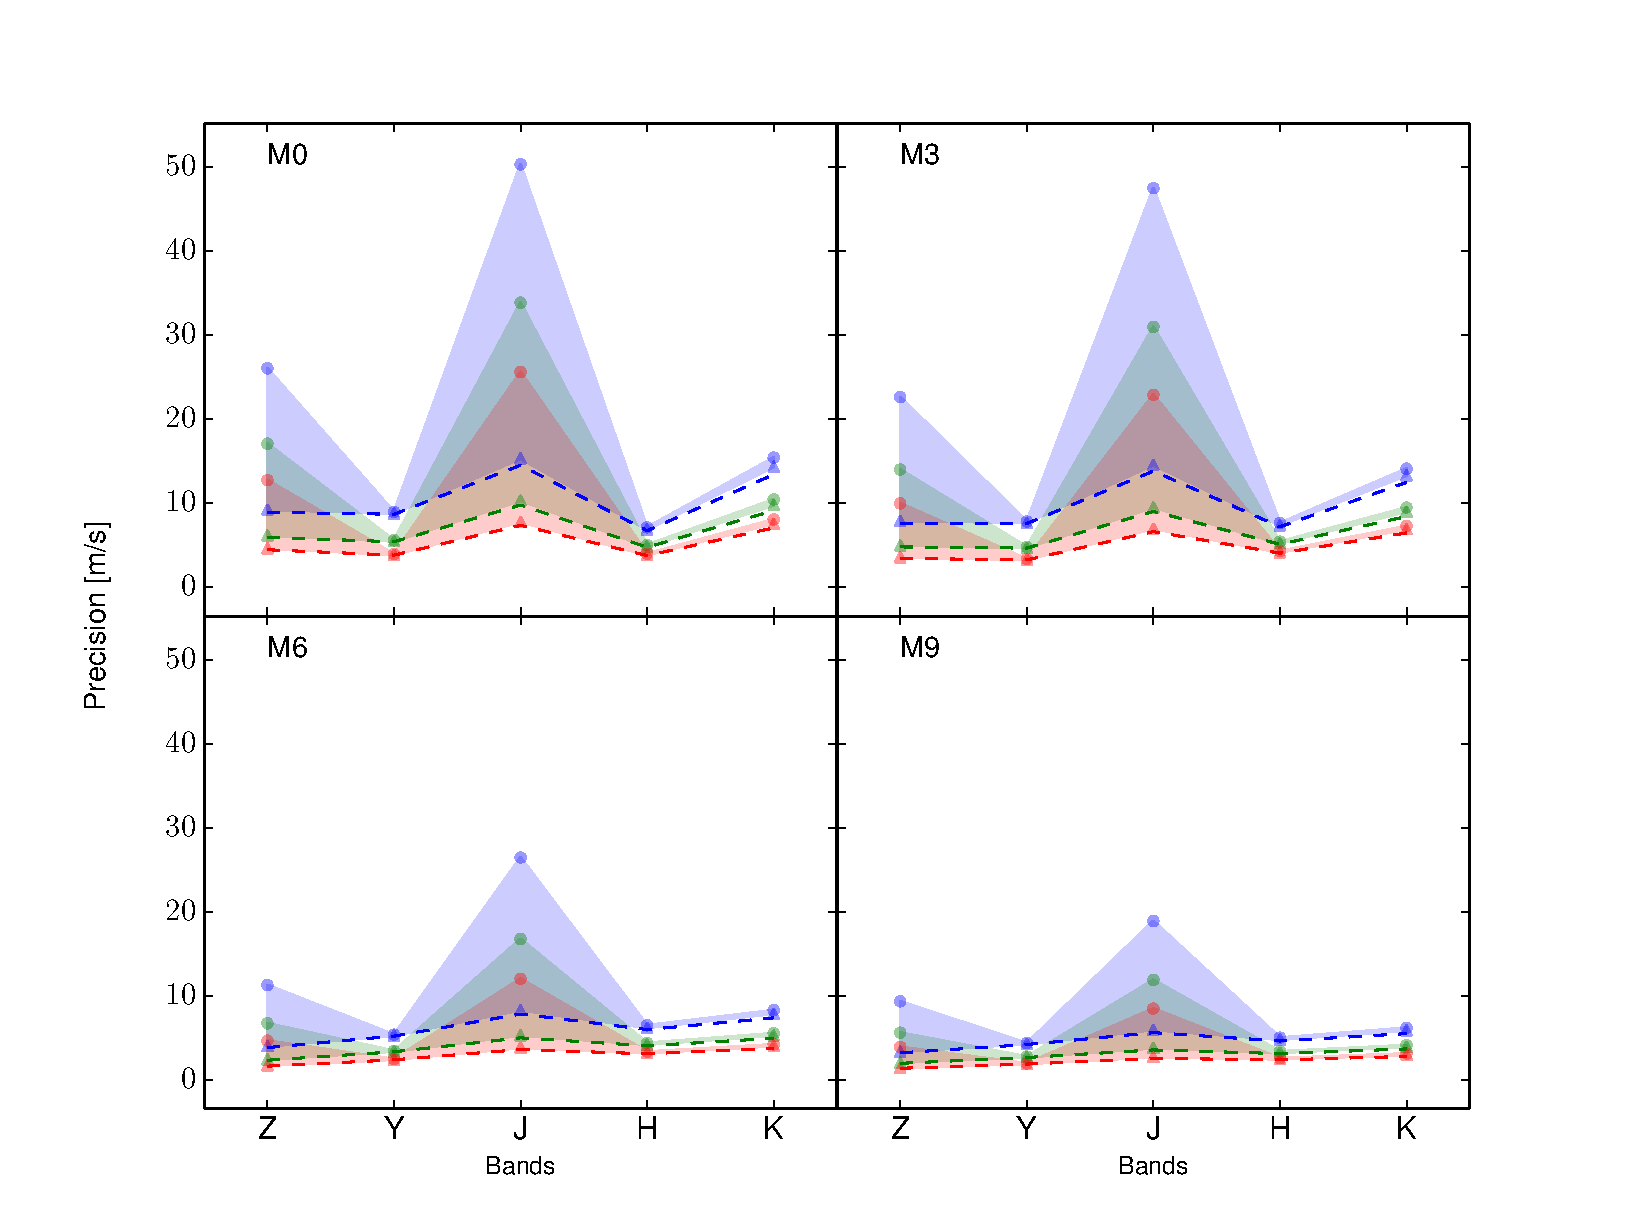
\includegraphics[width=0.48\linewidth]{figures/information-content/Rvprec_vsini1.pdf} &  % Figueria plot
        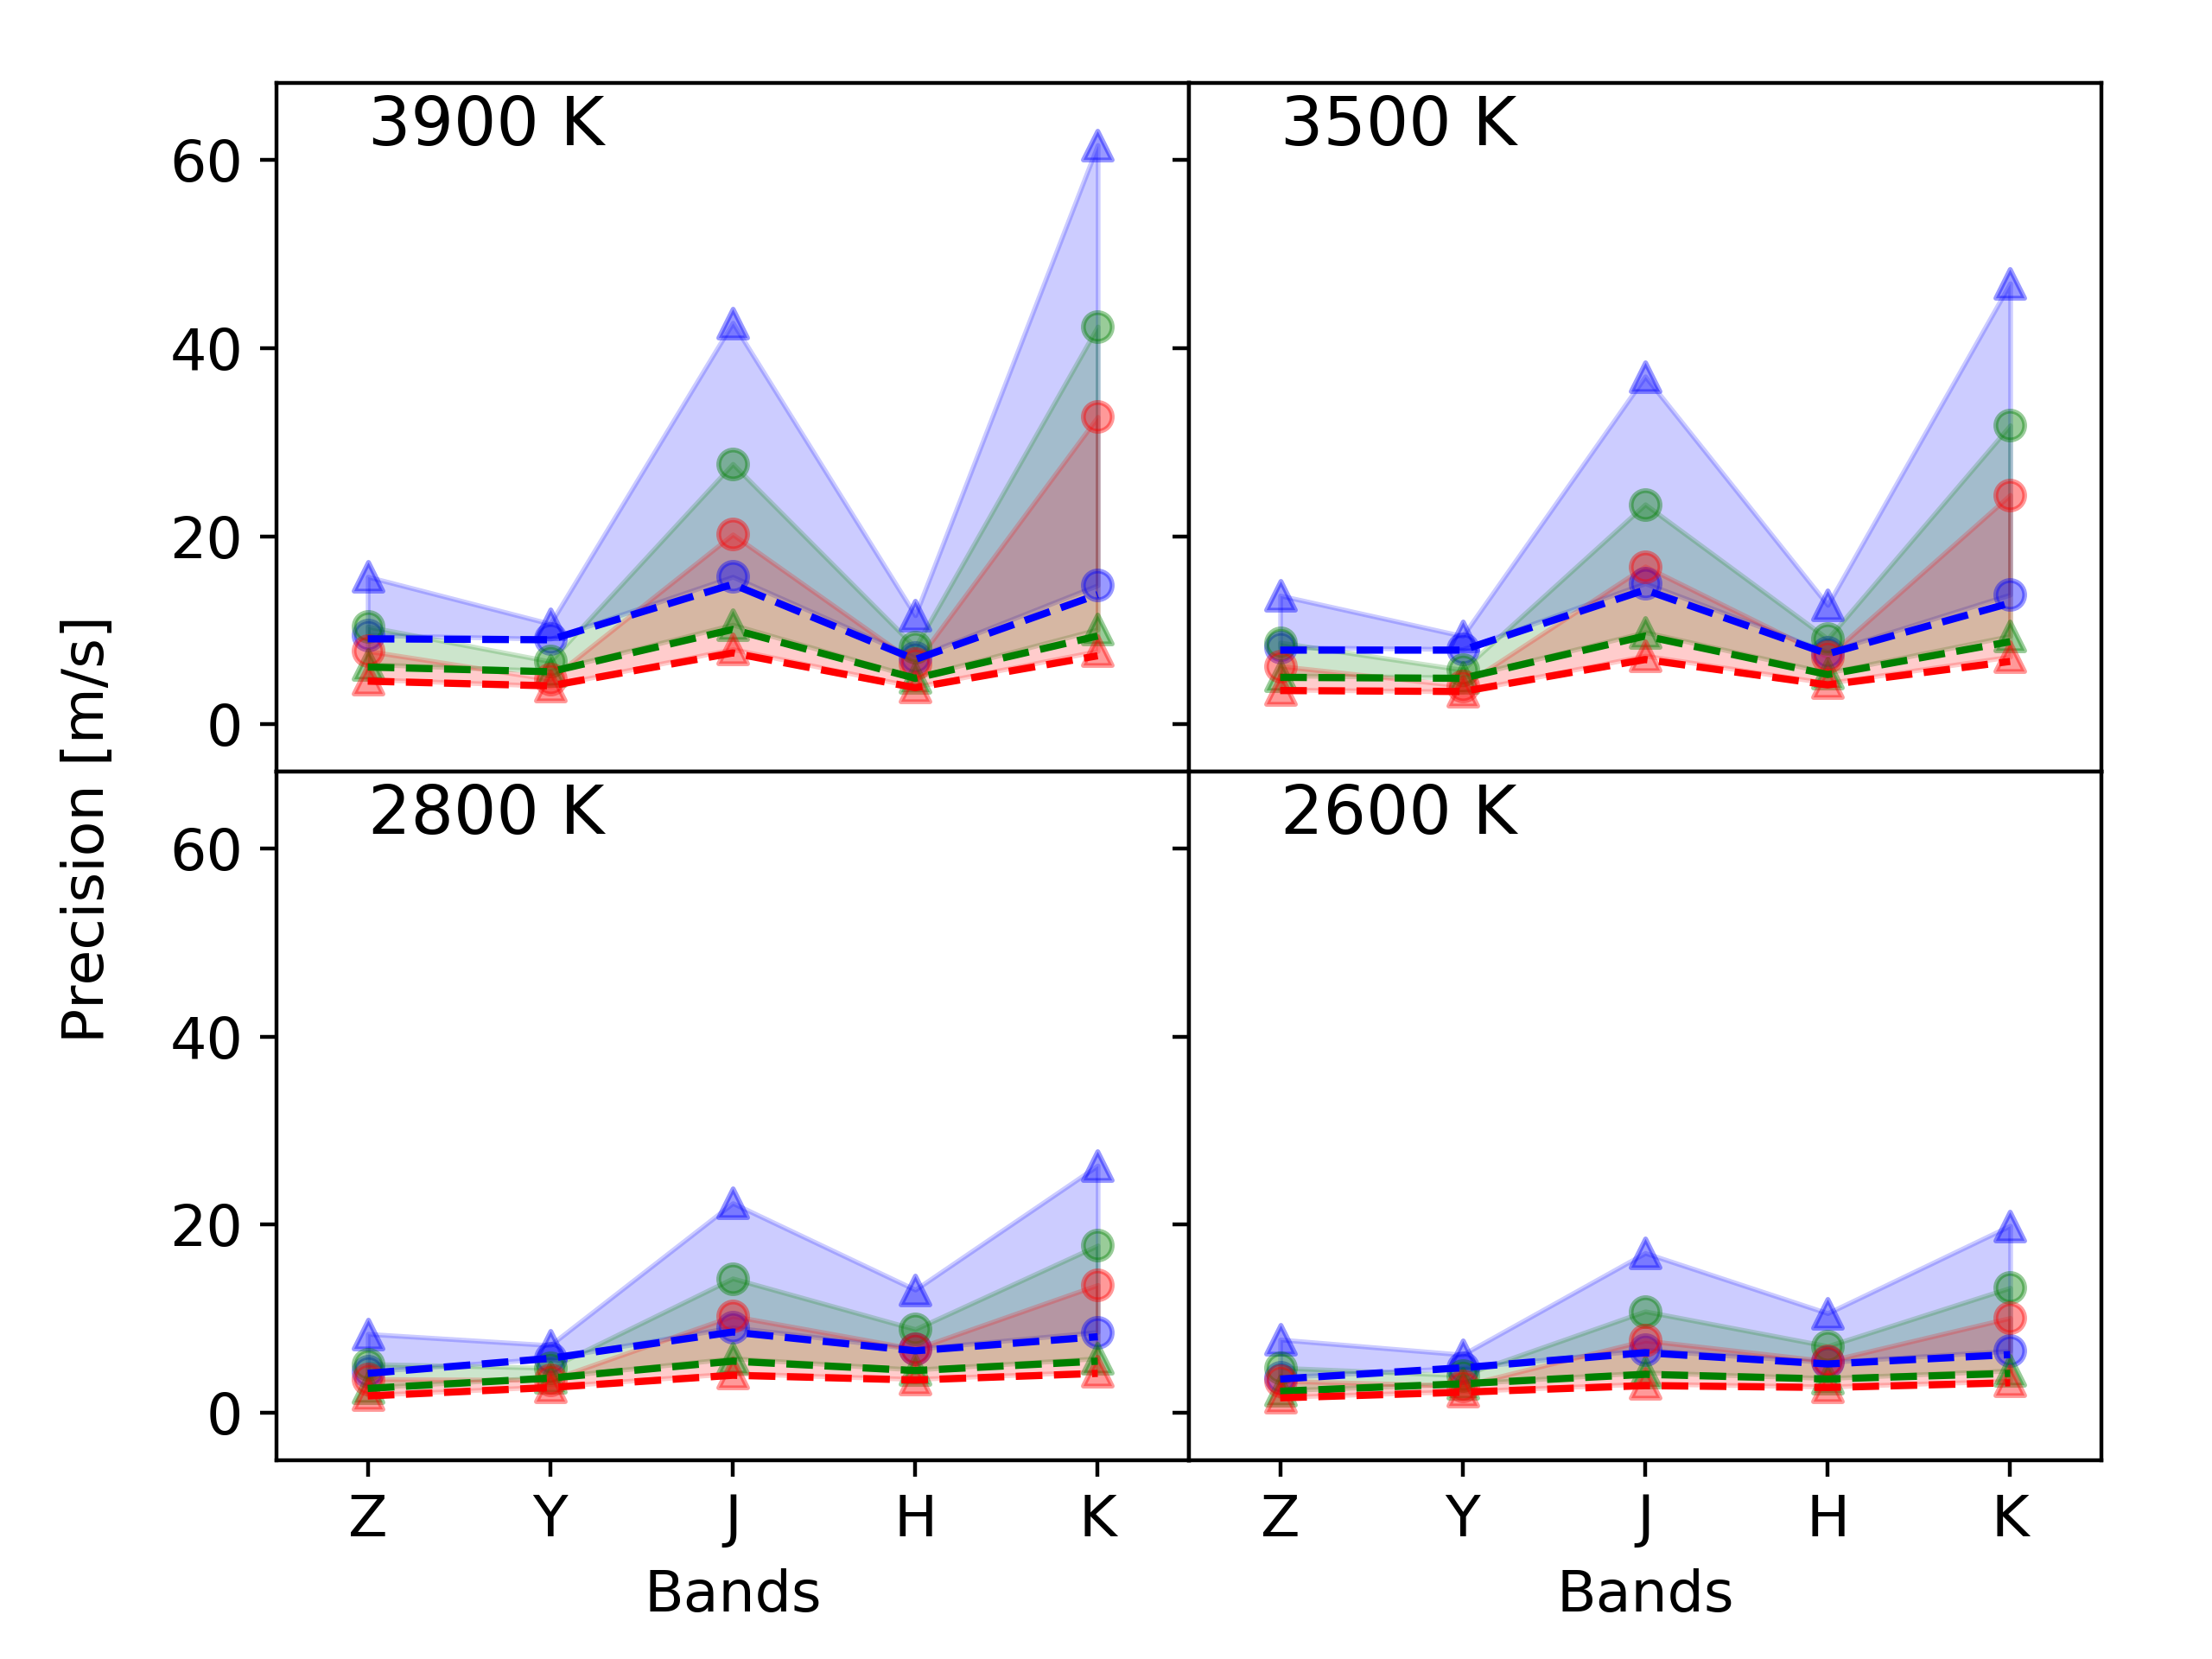
\includegraphics[width=0.47\linewidth]{figures/information-content/precision_fourpanel.png}\\ % eniric plot
    \end{tabular}
    \caption[Comparision of {RV} precision results to~\citet{figueira_radial_2016}.]{Comparison of the updated precision values.
        Each panel shows the precision achieved as a function of spectral band for stars with a rotational velocity of \Vsini=1.0\kmps{} and spectral types M0 (3900\K), M3 (3500\K), M6 (2800\K), and M9 (2600\K).
        The dashed line represents the theoretical limits imposed by Condition \#1, and the filled area represents the values within the limits set by Conditions~\#2 (circles) and \#3 (triangles); blue, green, and red represent the results obtained for resolutions of 60000, 80000, and 100000, respectively.
        The spectra were normalized to have a \snr{} of 100 per resolution element as measured at the centre of the \emph{J}-band.
        Left: Figure~1 from~\citet{figueira_radial_2016}.
        Right: Updated precision values computed using \emph{eniric}.
        The main difference is the area of shaded region due to the problem identified with Condition~\#2 (which is the upper edge).}
    \label{fig:figueria_comparision}
\end{figure}
\todo{Change to 55\mps{} upper limit?}


\section{Metallicity \Logg{} effects}
Here the affect of the metallicity and \Logg{} of the synthetic models in the {PHOENIX-ACES} library on the spectral quality of spectra.
This is achieved by using \eniric{} to compute the quality factor and RV precision for  \feh{} values between -1--1 and \Logg{} between 4.0--5.5.
In \cref{fig:deviations} the variation of quality factor with broadening of R=100\,000 and $\vsini=1.0$\kmps{} across the {M-dwarf} spectral types and the \nir{} bands is shown.
We observed multiple different effects present.


The \emph{Z}-band has a large separation in spectral quality due to spectral type, this is because the continuum the \emph{Z}-band is severely eroded in the spectra of late M's as they cool.
Each spectral type also behaves very differently to a change in \feh{} and \Logg{}.
For {M0} and {M3} there is an increase with \feh{} below solar metallicity, above solar metallicity the slopes of the lines dramatically increase, especially for {M3}.
For {M6} and {M9} there is a step slope with \feh{} below solar metallicity, which flattens off at solar metallicity, and even decreases for the {M9} spectra above solar metallicity.
As \Logg{} increases in the \emph{Z}-band there is a decrease in quality.
There is a consistently large separation between early and late M's that.
The quality for {M6} is very shallow, while for {M9} the quality is nearly flat for \Logg{}=4.0 and 4.5 but then decreases sharply at higher \Logg{}.

\emph{Y}-band -\\

\emph{J}-band - \\

For the H and \emph{K}-band there is fairly consistent linear trend for all spectral types, with the quality factor increasing with an increase in \feh{} and decreasing with an increase in \Logg{}.
There is also only a relatively small variation in quality factor due to the spectral type.


\begin{figure}
    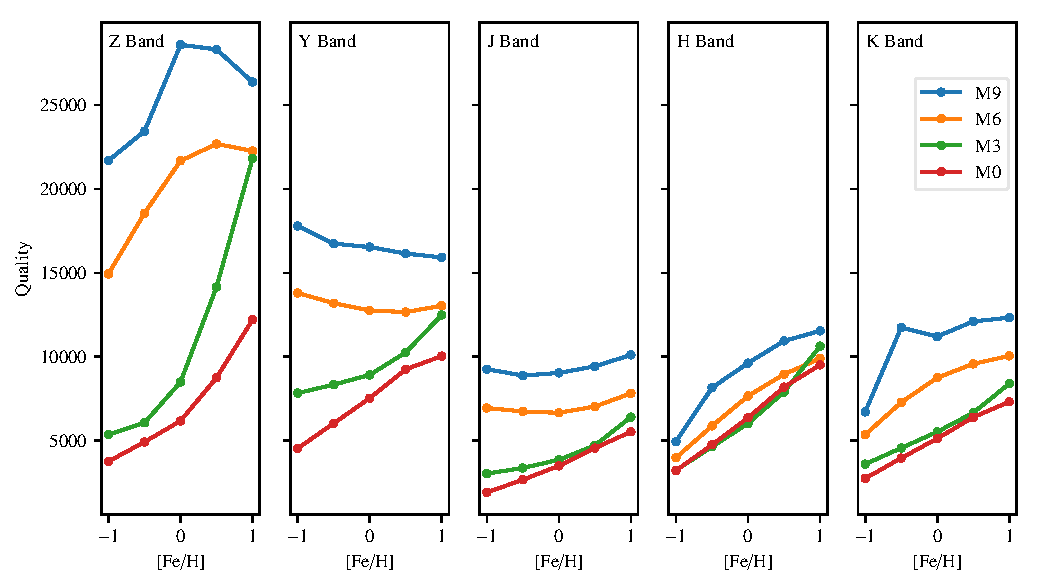
\includegraphics[width=0.99\linewidth]{figures/information-content/metalicity_effect.pdf}\\
    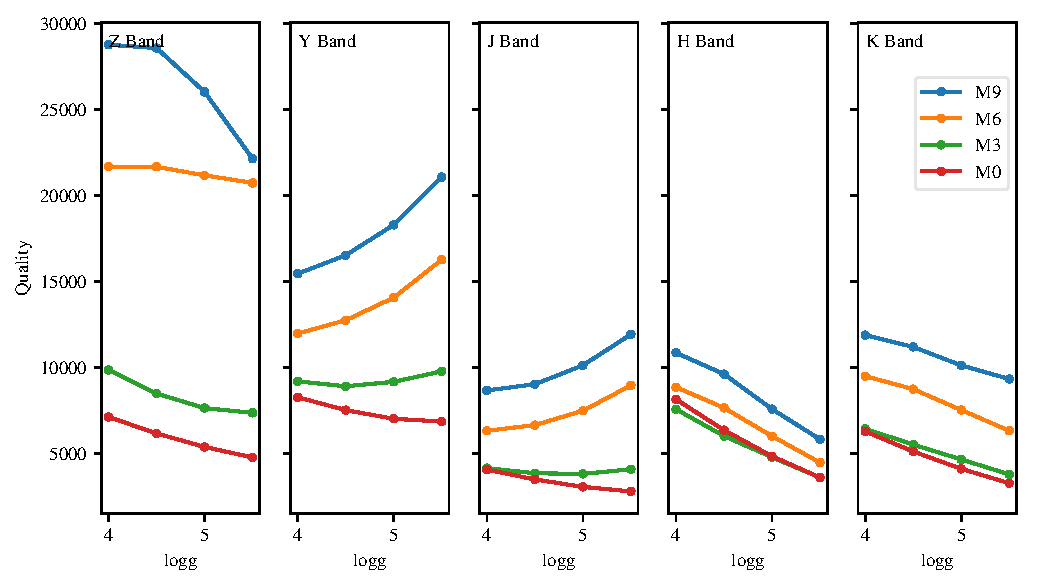
\includegraphics[width=0.99\linewidth]{figures/information-content/logg_effect.pdf}
    \caption[Quality factor verse \feh{} and \Logg{} for different spectral types and wavelength bands.]{Quality factor changes across spectral type and bands for variations in \feh{} and \Logg{}.
        Broadening values are R=100\,000 and \Vsini{}=1.0\kmps{}.
        Top: Quality factor variation of \feh{} between -1.0 to 1.0 at a fixed \Logg{}=4.5.
        Bottom: Quality factor variation of \Logg{} between 4 and 5.5 with fixed \feh{}=0.0.
        Note a higher quality factor corresponds to an increased {RV} precision.}
    \label{fig:deviations}
\end{figure}


\clearpage


\section{{SPIRou} and {NIRPS} {ETC}}\label{sec:spirou_nirps_etc}
Having this tool to calculate {RV} precisions efficiently lead to contributions to the Exposure Time Calculators (ETC) for both the {SPIRou} and {NIRPS} spectrographs.

In September 2017 \todo{we} were requested to provide precision calculations for the {SPIRou} ETC\footnote{\url{http://www.cfht.hawaii.edu/Instruments/SPIRou/SPIRou_etc.php}}.
These were the same table as~\citet{figueira_radial_2016} but with a each band referenced to 100~{\snr{}} in its own band.
The modification to use the centre of any band was made to fulfil this request.
Notes on the telluric correction issue affect on Condition~2.

In May 2018 \todo{we} were requested to provide precision calculations for the {NIRPS} {ETC}.\@ This extended the spectral range from {M0}, {M3}, {M6}, {M9} at 3900, 3500, 2800, 2600\K{} respectively, but to all temperatures between 2500 and 4000\K{} inclusively.
This provides a finer resolution coverage over the M spectral type, allowed by the {PHOENIX-ACES} library.
Instrumental resolutions of 75\,000 and 100\,000 were requested to match the {NIRPS} instrument.
The \Logg{} and metallicity, sampling rate remained at the~\citet{figueira_radial_2016} levels of 4.5, \textbf{0.0} and 3.0 respectively.\todo{}
Precisions were provided for \snr{} of 100 relative to the \emph{J}-, \emph{H}-bands as well as to each band individually.
Artigua 2018 (private communication 2018).\todo{Check how to cite priv communication properly}  suggested the truly relevant value is the \snr{} in \emph{H}-band for {NIRPS} radial velocities.

The results can be manually generated using ``eniric'' with the following incantation (after installation and configuration of {PHOENIX} library spectra.)
\textbf{A table of the precisions created for the {NIRPS} ETC are provided as an online table to \todo{our} publication} {Neal et al.
    2018b (in prep.)}\footnote{Review at \href{https://github.com/openjournals/joss-reviews/issues/1053}{https://github.com/openjournals/joss-reviews/issues/1053}.} \todo{Fix up when accepted}.


These values were both calculated and provided using the {FFD} gradient and with the incorrect masking order for Condition~\#2, splitting before calculating the pixel weights.
As \todo{we} demonstrated in \cref{sec:numerical_gradient,subsubsec:masking_order} these have a {RV} precision \(\sim\)2--7\% better than what would be computed with the current implementation.


\section{ metalicity / \Logg{} extension}




The incomplete telluric lines are the one of the largest contributors to the noise budget of extremely precise {RV} spectrographs~\citep{halverson_comprehensive_2016}, particularly the small mirco-telluric lines~\citep{cunha_impact_2014}.